\chapter{Introducción}
\label{cap1}

\section{Monitores de neutrones}
	Un monitor de neutrones es un detector de partículas provenientes del espacio, partículas de alta energía que inciden en la atmósfera terrestre. 
	Cuando una partícula proveniente del espacio penetra en la atmósfera esta choca con alguna de las partículas que forman la atmósfera. 
	Esta colisión genera muchas partículas secundarias, partículas que salen disparadas del violento choque y que a su vez 
	se chocan con otras partículas para dar lugar a aún más partículas segundarias. Vemos como una sola partícula proveniente del espacio produce el fenómeno 
	denominado cascadas atmosféricas. Como es de esperar con cada choque consecutivo se pierde parte de la energía que originalmente llevaba la 
	partícula extraterrestre, es muy normal que las partículas segundarias lleguen al nivel terrestre con tan solo 5\% de la energía que tenía la 
	partícula que originó todo el evento. Como es de esperar si una partícula no posee la energía suficiente la cascada no se propaga hasta la 
	superficie terrestre. Un monitor de neutrones es una estación terrestre que monitoriza la llegada de partículas extraterrestres de forma 
	indirecta a partir de las cascadas atmosféricas. Los monitores de neutrones están especialmente diseñados para capturar las partículas 
	secundarias producidas por la incidencia de partículas extraterrestres en nuestra atmósfera.
	\par
	La mayor parte de la radiación cósmica proviene de fuera de nuestro sistema solar, pero está fuertemente relacionada con 
	los ciclos solares. Los ciclos solares de 11 años aproximadamente, afectan la actividad solar pasando por un mínimo y un máximo, donde los
	cambios son apreciables en la luminosidad y el campo magnético \cite{SolarCicleWiki}. Es este segundo, el campo magnético solar, el que afecta a la llegada de 
	radiación cósmica a la Tierra. Al ser mayormente partículas con carga eléctrica, en la presencia de un fuerte campo magnético las partículas
	son desviadas, por lo que menos consiguen llegar a la Tierra cuando el campo magnético solar es más fuerte. A continuación detallaremos los
	sucesos más comunes que un monitor de neutrones registra. 
	\begin{itemize}
	  	\item	Ciclo solar. Como hemos explicado existe una fuerte relación entre la cantidad de radiación cósmica y la actividad solar. 
		  	La radiación cósmica es un buen indicador de la actividad solar donde la relación es inversa. Menos radiación generalmente
			significa una actividad solar elevada.	
		\item	Forbush decrease\cite{Forbush1938}. Estos sucesos consisten en un descenso rápido de los niveles de radiación cósmica medida en la Tierra. Estos
		  	descensos son consecuencia de CME's. La materia expulsada en un CME al ser en su mayoría plasma extiende e intensifica el 	
			campo magnético solar. Como ya hemos explicado el aumento del campo magnético solar conlleva al descenso de radiación cósmica. 
		\item	Ground level enhancements. Eventualmente la actividad solar es tan elevada que el Sol es capaz de emitir partículas
		  	suficientemente energéticas para que alcancen la superficie terrestre. Al alcanzar la superficie terrestre estas son 
			registradas por los monitores de neutrones lo que conlleva en un incremento brusco en la cantidad registrada. Estos sucesos
			son muy raros, entre 10 y 15 por década, aproximadamente.  
	\end{itemize}
	Para capturar estas partículas, en su mayoría protones y núcleos de Helio los monitores están compuestos por cuatro capas. Empezaremos 
	explicando primero la capa más exterior y acabaremos explicando la capa más interior.
	\begin{itemize}
		\item   Reflector. La primera capa consiste en un escudo reflector que tan solo deja pasar las partículas con energías altas. De 
		        esta manera todas las partículas generadas por el entorno inmediato que tienen baja energía rebotan y no influyen en nuestra 
			medición. 
		\item   Productor. La siguiente capa, generalmente de material denso tiene como objetivo conseguir algo parecido a las cascadas 
		        atmosféricas. La idea es tener un material denso para que sea muy probable que las partículas secundarias impacten con las partículas 
			del material y como resultado se produzcan más partículas. A las partículas generadas en esta capa se les da el nombre de
			neutrones de evaporación. Son estas partículas las que finalmente serán medidas por el instrumento, también son las que le dan
			nombre. Los neutrones producidos tienen menos energía, por lo que son más fáciles de medir. 
		\item   Moderador. A pesar de que las partículas que tenemos a este nivel tienen tan solo una fracción de la energía original estas
		        aún siguen siendo demasiado energéticas para ser capturadas. La siguiente capa tiene como objetivo ralentizar, disminuir 
			la energía, de las partículas para así poder capturarlas.
		\item   Contador. Un contador o tubo contador generalmente está relleno de gas ionizado con propiedades específicas. Cuando una de 
		  	las partículas ralentizadas por el Moderador choca con una de las partículas del gas es liberada una pequeña cantidad de
			energía en forma de electricidad, una señal eléctrica que podemos medir.
      	\end{itemize}
	Los sistemas de adquisición están diseñados para recoger estas pequeñas señales y medirlas. Tradicionalmente la medida que se realiza son 
	eventos por minuto, las señales son capturadas, amplificadas y registradas en un contador que se reinicia cada minuto. Con la realización
	del nuevo sistema de adquisición de datos nuestro objetivo es no tan solo proporcionar una dosificación de eventos sino proporcionar más 
	información sobre estos, en concreto mediremos la intensidad de las señales eléctricas. 


\section{NMDB}
	NMDB\cite{NMDB2011} es una red mundial de monitores de neutrones. Antes de proceder a hablar sobre la red en concreto expondremos las ventajas
	y razones de una red de monitores de neutrones.
	\begin{itemize}
		\item 	Espectro de energías. Al igual que el Sol, la Tierra tiene campo magnético. Este campo magnético repele con mayor fuerza en
		  	las regiones ecuatoriales que en los polos. Esto implica que solo las partículas más energéticas son perceptibles en las
			zonas ecuatoriales, mientras que en los polos las partículas no necesitan ser tan energéticas para alcanzar la superficie.
			Combinando dados de estaciones que se encuentran a diferentes latitudes podemos construir espectrogramas basados en la energía
			de las partículas.
		\item 	Anisotropía. Tener estaciones en diferentes lugares del globo terráqueo implica estar orientado a diferente dirección del
		  	espacio. Esto implica el poder hacer estudios sobre la procedencia de eventos.
		\item 	Redundancia. El tener muchas estaciones implica detectar el mismo evento en más de una estación. Esto nos permite comparar
		  	los datos entre estaciones y descartar fluctuaciones grandes, rápidas y asiladas en una sola estación.
		\item 	Cooperación. Estar en una red implica mejorar la comunicación entre las diferentes estaciones. De esta manera los resultados
		  	son mejores y el avance más rápido. 
	\end{itemize}
	Como ya hemos comentado NMDB es una red mundial, impulsada por la Comisión Europea. Actualmente la red supera las veinte estaciones. La red 
	proporciona datos en tiempo real con resolución de 1 minuto. Los formatos de los datos están estandarizados entre las diferentes estaciones.
	Los datos en tiempo real son utilizados para la elaboración de un sistema de alarma GLE\cite{GleAlarm}. Un GLE fuerte podría tener un impacto grande en
	nuestras vidas diarias, un impacto negativo. Es interesante poder detectar GLEs lo antes posible, este es uno de los objetivo de NMDB.
	Otro de los objetivos es hacer los datos fácilmente disponibles. Esto ha conllevado a que los datos de la red sean usados en otros campos 
	científicos no necesariamente relacionados con la radiación cósmica. 

\section{CALMA}
	CALMA\cite{Medina2013} es el primer y único monitor de neutrones en España y forma parte del NMDB. Dispone de 15 tubos contadores llenos con trifluoruro 
	de boro y un sistema de adquisición de datos que consiste en un sistema empotrado Linux que hace uso de una FPGA que es la encargada de 
	llevar las cuentas de los tubos. El sistema de adquisición actual ha sido desarrollado por el equipo de CALMA y también está implantado en 
	otras estaciones que forman parte del NMDB. La estación empezó a operar de forma plena de diciembre de 2012 y desde entonces lleva haciéndolo 
	ininterrumpidamente con pequeñas excepciones. El equipo técnico a cargo de la estación está profundamente implicado en desarrollar sistemas y herramientas 
	que mejoren el funcionamiento del NMDB. La idea para este trabajo es desarrollar el software del nuevo sistema de adquisición que el equipo 
	de CALMA está desarrollando, una vez realizado el nuevo sistema de adquisición desarrollaremos una herramienta que nos permitirá monitorizar 
	el estado de nuestra estación.
	Desde su puesta en marcha la estación ha registrado 18 Forbush decreases. Desafortunadamente aún no ha habido ningún GLE que detectar, aunque este
	tendría que ser muy energético para ser detectado en una estación con tan poca latitud. 
	Procederemos a hablar más a fondo del estado actual de CALMA, hablaremos del sistema de adquisición, base de datos, herramientas y técnicas
	que son usadas.
	\subsection{Sistema de adquisición}
		Actualmente el sistema de adquisición que está implantado en CALMA es producto del propio equipo\cite{Garcia2014}. El sistema consiste en un sistema empotrado
		Linux que hace uso de una FPGA que procesa las señales procedentes de los tubos. Antes de llegar a la FPGA las señales pasan por un circuito 
		de adaptación, las señales pasan de analógicas a digitales. La FPGA se encarga de llevar la cuenta del número de eventos para los 18 canales. El 
		software que se ejecuta en el sistema Linux tiene como tarea comunicarse con la FPGA, recoger las cuentas de cada minuto y finalmente guardar los
		datos en una base de datos.  
		\par 
		El nuevo sistema que se está diseñando a grandes rasgos sería lo mismo, un sistema empotrado Linux con una FPGA. La idea es que el nuevo sistema
		de adquisición sea muy flexible, pueda suportar diferentes tubos, barómetros y otros periféricos. Esta flexibilidad nos permitirá implantar 
		fácilmente este sistema en otras estaciones. El sistema también está pensado para futuramente ser extendido y poder procesar información 
		procedente de detectores de muones. Aparte de la flexibilidad el nuevo sistema de adquisición incorporara funcionalidades extra, supervisara
		variables que afectan al proceso de adquisición y antes no se tenían en cuenta.
	\subsection{Bases de datos}
		Actualmente la base de datos que genera CALMA está diseñada de acuerdo con el estándar impuesto por NMDB. Actualmente existen dos réplicas
		de la base de datos. Tenemos una réplica de los datos crudos adquiridos en el propio sistema, para gestionar esta réplica utilizamos Sqlite3. La
		segunda réplica está en otra máquina conectada por red con el sistema de adquisición de datos. La segunda réplica contiene los datos crudos y 
		también contiene la corrección por presión de estos. Para la segunda réplica usamos MySQL. Los datos que mandamos al NMDB son los datos de la 
		segunda réplica.
	\subsection{Herramientas y técnicas}
		Actualmente el equipo de CALMA hace uso de herramientas que les ayudan a analizar la información desde el punto de vista científico. Estas 
		herramientas están muy bien para los científicos, pero actualmente no existe ninguna herramienta que nos dé información sobre el estado técnico 
		de la estación. Nuestra idea es crear una herramienta Web para poder automatizar algunas de las tareas que ahora son realizadas manualmente. 


\section{Objetivos}
	El objetivo de este proyecto es desarrollar el software para el nuevo sistema de adquisición de datos y también desarrollar una herramienta
	que nos permita operar y monitorizar el estado de la estación. 
	\subsection{Software adquisición de datos}
		Actualmente El equipo de CALMA está desarrollando un nuevo sistema de adquisición de datos para su estación. Como comentamos
		anteriormente este estará basado en un sistema empotrado Linux. En ese entorno Linux se ejecutara el software de adquisición. El software
		es el encargado del correcto funcionamiento de los demás componentes que forman el sistema de adquisición. A grandes rasgos
		el software deberá cumplir los siguientes objetivos.
		\begin{itemize}
			\item 	Coordinar la estación. El objetivo principal es coordinar la estación y todos los módulos que la componen. El software
			  	debe ser capaz de configurar los demás módulos, pedirles la información que generan y guardar esta en una base de datos. 
			\item 	Iniciar automáticamente la estación. Una vez configurado adecuadamente, ante la presencia de corriente eléctrica, el
			  	software debe ser capaz de arrancar automáticamente la estación, esto implica configurar y sincronizar los demás
				módulos. Las ventajas de que el arranque sea automático son muchas y muy fáciles de concebir.
			\item 	Detectar estados anormales. El software debe ser capaz de detectar cuando no está funcionando según lo previsto. En
			  	una estación de este tipo funcionar mal la mayoría de veces es no generar datos o generar datos anormales. Ante la
				presencia de un estado anormal el software debe generar algún tipo de alerta y si es posible intentar solucionar el
				problema que en la mayoría de las veces consiste en realizar un reinicio.
		\end{itemize}
		Uno de los objetivos de este trabajo es realizar, implantar y mantener este software de adquisición. Los demás módulos son desarrollados
		por el equipo de CALMA. El autor de este trabajo no ha formado parte en el desarrollo de estos, pero a lo largo de este trabajo se
		describirán las interfaces de estos, dado que es necesario para entender este trabajo. 
	\subsection{Herramienta Web}
		El segundo objetivo de este trabajo es el desarrollo de una herramienta que facilite la gestión de una estación. La idea de esta
		herramienta es del equipo de CALMA. Procederemos a detallar las funcionalidades de la herramienta tal y como la concibe el equipo de
		CALMA.
		%TODO Citar el artículo de la herramienta.
		\begin{itemize}
	         	\item	Spike Tool. Módulo que nos permita la detección de Spikes. Usando los datos proporcionados por el sistema de
			  	adquisición este módulo debe generar gráficos. Estos gráficos serán interactivos y su propósito será hacer fácil la
				detección de Spikes. Los Spikes detectados podrán ser marcados como nulos en el conjunto de datos revisados. 
			\item 	Configuración de la estación. Este módulo nos permitirá cambiar la configuración de la estación en tiempo real. Nos
			  	permitirá desconectar tubos contadores, lo que viene muy bien si se detecta algún tubo que está funcionando mal. Este
				módulo se comunicaría directamente con el software de adquisición. 
			\item 	Estadísticas Online. Módulo que calculara estadísticas en tiempo real. Esto nos permitirá detectar problemas y en
			  	consecuencia aplicar las acciones necesarias. 
			\item	Alertas. La herramienta debe generar alertas cuando se detectan comportamientos no deseados, por ejemplo la
			  	herramienta tendría que generar una alerta cada vez que se detecta que no se están generando datos.
			\item 	Histogramas con la intensidad de los eventos. El nuevo sistema de adquisición proporciona información sobre la energía
			  	de las partículas incidentes. Este módulo debería generar histogramas con estos datos. Estos histogramas nos
				permitirían hacer mejores diagnósticos sobre el funcionamiento de los tubos contadores. 
		\end{itemize}
		Podemos ver que la herramienta ofrece un gran abanico de funcionalidades, por desgracia en este trabajo tan solo nos centraremos en el
		primer módulo. Realizar los demás módulos estaría fuera del alcance de un trabajo como este. También es de destacar que tan solo
		nos centraremos en la implementación, no implantaremos ni mantendremos la herramienta. La herramienta será una herramienta Web 
		intuitiva y altamente interactiva. 
		

\section{Diseño preliminar}
	\subsection{Software de adquisición}
		Procederemos a especificar un diseño preliminar del software de adquisición. El software se ejecutara en un sistema empotrado Linux sobre
		una BeagleBone Black. La distribución elegida para desarrollar este trabajo es Ångström, la que viene por defecto con la BeagleBone
		Black. Actualmente nos estamos planteando cambiar la distribución a alguna derivada de Debian, sobre esto hablaremos más a fondo en el
		capítulo \emph{Conclusiones y Trabajos futuros}. El desarrollo del software se hará en Python. Hemos elegido Python por gustos
		personales, detrás de esta elección no hay algún motivo relevante. Para la gestión de la base de datos hemos elegido Sqlite3,
		Sqlite3 es una elección popular en sistemas empotrados como el que estamos realizando. 
		\par
		En la figura \ref{fig:soft_control_preliminar} podemos ver el diseño preliminar de nuestro software. Al iniciar lo primero que 
		tiene que hacer es configurar la estación. Esto implica configurar a los demás módulos y también configurarse a sí mismo. Si la
		configuración no ha sido exitosa procedemos a reintentarlo y si es posible notificar el fallo. Si la configuración ha sido exitosa pasamos al
		funcionamiento nominal, adquisición de datos. El funcionamiento nominal consiste en registrar los valores medidos cada minuto. Los
		valores de cada minuto son entonces guardados en una base de datos local.
		\begin{figure}[h]
			\centering
			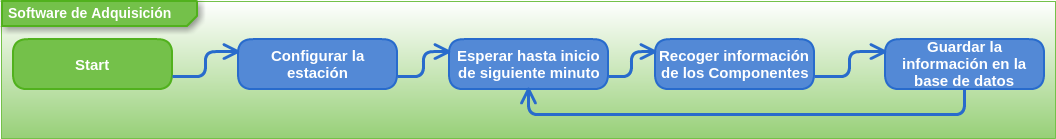
\includegraphics[keepaspectratio, width=1\textwidth]{./img/soft_control_preliminar.png}
			\caption{Software de adquisición. Diseño preliminar.}
			\label{fig:soft_control_preliminar}
		\end{figure}
	\subsection{Herramienta Web}
		En la figura \ref{fig:herramienta_web_preliminar} podemos ver el diseño de nuestra App. Como podemos ver el diseño está fuertemente basado en el patrón
		MVC\cite{MVCWiki}. A continuación explicaremos los tres componentes básicos. 
		\begin{description}
			\item[Base de Datos]    En este componente residen los datos de nuestra estación. Para la gestión de estos utilizamos un servidor MySQL.
			\item[Back-end]    	Este componente es el encargado de recibir y procesar las solicitudes provenientes del Front-end. Una vez procesadas
			  			las solicitudes si estas son válidas este componente se comunica con la base de datos para ejecutar las solicitudes. 
						Por último devuelve los resultados de las solicitudes. Para la implementación de este componente hemos utilizado
						ZendFramework y Apygility.  
			\item[Front-end]    	Este componente implementa la interfaz de nuestra aplicación. Es el encargado de presentarnos la información y
			  			manejar las peticiones del usuario. El módulo está basado en el patrón MVC. Para implementar la Vista hemos
						utilizado HighStock, para el Controlador ExtJs y para el modelo peticiones Ajax.
		\end{description}
		\begin{figure}[h]
			\centering
			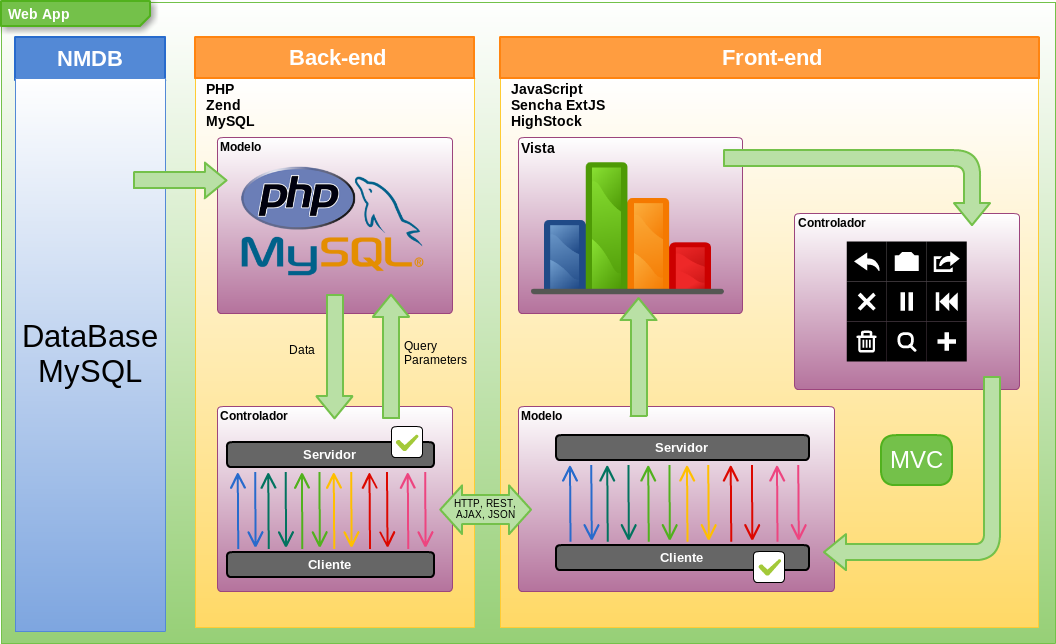
\includegraphics[keepaspectratio, width=1\textwidth]{./img/herramienta_web_preliminar.png}
			\caption{Herramienta Web. Diseño preliminar}
			\label{fig:herramienta_web_preliminar}
		\end{figure}
\section{Proceso de adquisición}
	\subsection{Overview general}
		Procederemos a explicar más a fondo el proceso de adquisición, haremos hincapié en los aspectos más relevantes para este trabajo. Empezaremos
		por los tubos contadores y terminaremos por los datos generados y su significado.
		\par
		Como ya comentamos, la radiación cósmica termina generando neutrones de baja energía. Son estas partículas las que interaccionan con el gas de
		los tubos contadores, en el proceso es liberada una pequeña cantidad de energía. Esta pequeña cantidad de energía es capturada en forma de
		señal eléctrica. Las señales resultantes son muy pequeñas, por lo que estas pasan por un circuito de adaptación. 
		\par
		En el circuito de adaptación las señales son amplificadas y digitalizadas. En el sistema de adquisición actual para cada señal el circuito
		de adaptación genera un pulso fijo. El nuevo sistema de adquisición incorpora nuevo circuito de adaptación. Este nuevo circuito de
		adaptación genera un pulso cuyo ancho de banda es proporcional a la energía de la señal. 
		\par
		Las señales generadas por el circuito de adaptación son dirigidas a la FPGA. La FPGA procesa las señales entrantes, para cada pulso recibido
		registra un evento y además mide el ancho del pulso. La información es entonces transmitida a la BeagleBone Black, a nuestro software de
		adquisición. Más adelante en este trabajo explicaremos la interfaz de comunicación entre la BeagleBone y la FPGA, en este punto la vamos a omitir. 
		\par
		Como hemos podido ver la información de los eventos termina en manos de nuestro software de adquisición. El software se encarga de recibir
		correctamente dicha información y de guardarla en una base de datos con resolución de 1 minuto.
	\subsection{Múltiples Tubos}
		Hasta ahora siempre hemos hablado de tubos contadores, en plural, detrás de esto hay una razón. Normalmente las estaciones se componen de
		varios tubos contadores, donde 18 tubos contadores es un estándar. Vamos a explicar el motivo de tener muchos tubos contadores. 
		\par
		Cuando un tubo contador registra un evento, es porque una partícula de alta energía ha impactado con la atmósfera terrestre. La cuestión está
		en que desde ese primer impacto hasta que se registra un evento en el tubo contador entremedias hay una serie de eventos cada uno con una
		probabilidad asociada. No hemos hablado mucho de estas probabilidades así que continuación detallaremos algunas, para poder hacernos una idea. 
		\begin{itemize}
			\item Productor. 	Una partícula que llega al productor tiene cierta probabilidad de interactuar con este o no. Si dicha
			  			interactuación se produce se generaran neutrones que medir.
			\item Contador. 	Un tubo contador tiene una cierta probabilidad de detectar un neutrón o no hacerlo. Si el neutrón se detecta
			  			se registraría un evento.
		\end{itemize}
		Como vemos detectar una partícula depende de muchos eventos probabilístico, por lo tanto es en sí mismo un evento probabilístico. Tener tan
		solo un tubo no sería práctico, los datos tendrían gran dispersión. La solución de este problema es tener mucho tubos, cuantos más mejor.
	\subsection{Valores globales y correcciones}
		Tener los datos de muchos tubos es bueno, sin embargo no es muy práctico trabajar con esos datos en crudo. Tener un valor global de toda la
		estación es más representativo. Es por eso por lo que el sistema de adquisición calcula uno a partir de los datos de todos los tubos. Hay 
		diferentes modos de calcular este valor global y es algo que está en continua discusión. Nosotros también vamos a calcular este valor, 
		utilizaremos el Median Algorithm\cite{MedianAlgr}.
		\par
		Anteriormente hemos comentado que también medimos el valor de la presión atmosférica. Medimos este valor porque es útil. Ya hemos explicado
		las cascadas atmosféricas donde partículas de la atmósfera chocan unas con otras. Tener diferentes niveles de presión atmosféricas afecta a
		las cascadas atmosféricas, en consecuente a la cantidad de partículas que llegan a la superficie terrestre, a menos presión, más partículas,
		y a más presión, menos partículas. Resumiendo este último párrafo  podemos decir que el valor global sin corregir es un indicativo de cuanta
		radiación cósmica llega a la superficie terrestre, y el valor corregido en función de la presión es un indicativo de cuanta radiación cósmica
		llega a nuestra atmósfera.
	\subsection{Fuentes de alimentación de alta tensión}
		Para funcionar los tubos contadores es necesaria una corriente de alta tensión y baja intensidad. La corriente es utilizada por los tubos
		para ionización del gas dentro del tubo. La ionización del gas afecta al funcionamiento de los tubos, por lo que cambios en la corriente
		subministrada pueden afectar al sistema de adquisición. Es por esta razón por la que el funcionamiento de las HVPS es supervisado. Es de esperar
		que la corriente sea constante, por lo que no es necesaria ninguna corrección en función de esta. En caso de variaciones en la corriente los datos
		generados son considerados no consistentes.
